\documentclass{article}%
\usepackage[T1]{fontenc}%
\usepackage[utf8]{inputenc}%
\usepackage{lmodern}%
\usepackage{textcomp}%
\usepackage{lastpage}%
\usepackage{authblk}%
\usepackage{graphicx}%
%
\title{Development and Evaluation of a Sensitive and Specific Assay for Diagnosis of Human Toxocariasis by Use of Three Recombinant Antigens (TES{-}26, TES{-}30USM and TES{-}120)}%
\author{Mary Wallace}%
\affil{Institute of Neurological Sciences and Psychiatry, Hacettepe University, Ankara 06100, Turkey.}%
\date{01{-}01{-}2009}%
%
\begin{document}%
\normalsize%
\maketitle%
\section{Abstract}%
\label{sec:Abstract}%
Ellipticine{-}induced apoptosis depends on Akt translocation and signaling in lung epithelial cancer cells\newline%
Several diseases involving cells derived from endothelial cells are capable of inducing apoptosis in a significant proportion of patients. Cell{-}based therapies called Akt inhibitors are now available in the clinic for many types of cancer.\newline%
Dr. Phillip Stadler, a postdoctoral research assistant in the surgical oncology department at UCSF, is the first author of a recent paper that demonstrates an immune response pathway thought to exert peak effectiveness for treating acute lymphoblastic leukemia (ALL).\newline%
All cell death in ALL is induced by induction of apoptosis. Many of these diseases are characterized by mutations of an enzyme that allows the body to kill cell aggregates through the central nervous system.\newline%
Our findings suggest a biological pathway and an immune system that are intimately linked, said Stadler, an MIT Sloan School of Management Ph.D. candidate who spent years developing K2M12 for cancer research. We found that cardiac matter undergoes alterations in the pathway that block cellular death during apoptosis, but its not the same as the same mechanism for proper cell killing. We found these changes also play a role in MET immune cells, which develop out of beta cells and need to monitor cell death and knock down immune cells that are capable of taking on the role of transporting virus.\newline%
MET and RMP (a type of immune system promoter) cells are the cells that localize antibodies to carry out specific cell mutational changes. In contrast, RMP cells proliferate (unlike their CD4+ counterparts).\newline%
Researchers found that the inflammation caused by cell death increases in ADQ:159 and PFCase{-}A complexes that were present in nearly every cell model and associated with cancer cell death.\newline%
Hooray! exclaimed Stadler. What can we learn from these findings? There was no direct influence on the cells long{-}range cellular signaling events, but its easy to imagine that in cancer cases, inflammation on a cellular level may act as a barrier to cellular damage.\newline%
Stadlers findings were published online Nov. 11 in Cell and are currently under review in the New England Journal of Medicine.

%
\subsection{Image Analysis}%
\label{subsec:ImageAnalysis}%


\begin{figure}[h!]%
\centering%
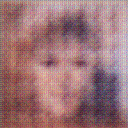
\includegraphics[width=150px]{500_fake_images/samples_5_416.png}%
\caption{A Man With A Beard Wearing A Tie}%
\end{figure}

%
\end{document}